\chapter{Using the Software System}
\label{appendix:software_usage}
The following chapter gives a tutorial on how to use the software system (see Chapter~\ref{software_system}) implemented to conduct the experiments in this thesis.

\section{Download}
The code of the software system can be downloaded by using \texttt{git}\footnote{https://git-scm.com/}. The repository is located on the publicly accessible GitHub website\footnote{https://github.ch/vongrdir/BA-ML-17}. However, the visibility of the repository is set to private. To gain access, please send an e-mail with the request and the username of your GitHub account to either \texttt{vongrdir@students.zhaw.ch} or \texttt{weilemar@students.zhaw.ch}.

\section{Requirements}
To use the software and all the related scripts, the following software packages must be installed:

\begin{itemize}[noitemsep]
	\item \texttt{python} in the version 3.5.2\footnote{https://www.python.org/}
	\item If a GPU is used:
	\begin{itemize}[noitemsep]
		\item Nvidia GPU driver\footnote{http://www.nvidia.de/Download/index.aspx} for the respective GPU.
		\item Nvidia \texttt{cuda} 8 toolkit\footnote{https://developer.nvidia.com/cuda-toolkit}.
	\end{itemize}
\end{itemize}

The experiments and script can also be conducted without a GPU and solely on the CPU. However, this leads to higher runtime in several parts of the system, mainly when training models. In addition to the mentioned software packages the \texttt{python} libraries listed in Chapter~\ref{software_system:software_packages} must be installed.

The libraries can be installed via the \texttt{python} package manager \texttt{pip}\footnote{https://packaging.python.org/installing/}. It is recommended to us the exact versions of the mentioned software packages and \texttt{python} libraries to avoid any compatibility issues. However, it might certainly be possible that the software system runs find with newer version without any problems.

\clearpage
\section{Structure of the Repository}
In the following table, we explain the structure of the repository and the contents of the main directories.

\begin{table}[H]
	\centering
	\begin{tabularx}{\textwidth}{lX}
		\toprule
		Name of Directory & Description\\ \midrule
		\texttt{configs/} & In this directory, all the JSON configurations for all experiments are stored.\\
		\texttt{report/} & All documents related to the thesis are stored in this directory.\\
		\texttt{misc/} & Directory for storing miscellaneous files.\\
		\texttt{results/} & The results of all the run experiments are stored in this directory. The results themselves are stored in a directory named after the \texttt{WHAT} of the experiment. In total, the model, all collected metrics and the configuration of experiments are stored in this directories.\\
		\texttt{scripts/} & The scripts used in this thesis are stored in this directory (see Chapter~\ref{software_usage:using_scripts}).\\
		\texttt{source/} & The whole source code of the software system itself is located in this directory including all the components necessary to implement the system described in the Chapter~\ref{sofware_system}.\\
		\bottomrule
	\end{tabularx}
	\caption{Remarks regarding the structure of the repository.}
\end{table}
\todo{update}

\clearpage
\section{Using the Scripts}
\label{software_usage:using_scripts}
In the following section, we are going to introduce the most important scripts necessary to use the software system for running experiments. The scripts themselves are located in the directory \texttt{scripts/}.

\begin{table}[H]
	\centering
	\ra{1.3}
	\begin{adjustbox}{max width=\textwidth}
		\begin{tabular}{lp{8cm}p{8cm}}
			\toprule
			Name & Description\\ \midrule
			\texttt{analyse{\_}ngram{\_}from{\_}corpus.py} & With this script, it is possible to analyse a corpus regarding its bigrams. This script was used to generate the n-grams in Chapter~\ref{chapter:data:ngram} and~\ref{results:development_language_model}.\\
			\texttt{analyze{\_}timestamp{\_}problematic{\_}opensubtitles.py} & With this script, the time-lag analysis between utterances in the OpenSubtitles corpus can be done (see Chapter~\ref{data:opensubtitles:time_lag_analysis}).\\
			\texttt{analyze{\_}word{\_}coverage.py} & This script allows to analyse the word coverage of a corpus with regard to a given vocabulary (see Chapter~\ref{data:word_coverage}).\\
			\texttt{split{\_}corpus.py} & This script allows to split a given corpus into a training, test and validation set by proportions. The split itself is done randomly (see Chapter~\ref{data:split_corpus}).\\
			\texttt{evaluate{\_}trained{\_}model.py} & This script allows to evaluate a trained model on a certain dataset and stores the resulting metrics of this evaluation.\\
			\texttt{generate{\_}s2v{\_}sequence{\_}embeddings.py} & This script allows for generating Sent2Vec embeddings for the given list of sequence samples. These are then used in Chapter~\ref{results:performance_on_test_datasets} for the similarity analysis.\\
			\texttt{get{\_}internal{\_}embeddings{\_}from{\_}samples.py} & This script allows to generate thought vectors for a list of given sample texts. They are used in the analysis in Chapter~\ref{results:thought_vector_clustering}.\\
			\texttt{preprocess{\_}opensbutitles{\_}data.py} & This script is responsible for preprocessing the raw OpenSubtitles corpus as described in Chapter~\ref{data:preprocessing}.\\
			\texttt{preprocess{\_}reddit{\_}corpus.py} & This script is responsible for preprocessing the raw Reddit corpus and building the tree which is the finally converted into the datasets as described in Chapter~\ref{data:preprocessing}.\\
			\texttt{talk{\_}to{\_}model.py} & This script provides a possibility to talk to trained models through the terminal. The functionality is basically the same as in the web frontend (see Chapter~\ref{sofware_usage:web_frontend}).\\
			\bottomrule
		\end{tabular}
	\end{adjustbox}
	\caption{Descriptions of the most important scripts to use the software system.}
\end{table}
\todo{update}

There are much more scripts than the ones described above (e.g. for plotting, creation of vocabularies). Not all of them are necessary to conduct experiments, which is why only explain the most important.

In the following table there are exemplary calls for all scripts listed above:

\begin{table}[H]
	\centering
	\ra{1.3}
	\begin{adjustbox}{max width=\textwidth}
		\begin{tabular}{lp{20cm}}
			\toprule
			Name & Exemplary Call\\ \midrule
			\texttt{analyse{\_}ngram.py{\_}from{\_}corpus.py} & python scripts/analyse{\_}ngram.py{\_}from{\_}corpus.py data/opensubtitles/opensubtitles\_raw.txt 2 results/opensubtitles/bigram\_analysis.csv results/opensubtitles/bigram\_analysis\_words.csv\\
			\texttt{analyze{\_}timestamp{\_}problematic{\_}opensubtitles.py} & python scripts/analyze{\_}timestamp{\_}problematic{\_}opensubtitles.py data/OpenSubtitles2016 analysis\_timestamps\_opensubtitles.json\\
			\texttt{analyze{\_}word{\_}coverage.py} & python scripts/analyze{\_}word{\_}coverage.py data/reddit/reddit\_corpus.txt word\_coverage\_reddit\_new.json data/reddit/vocab\_100k.pickle,data/reddit/vocab\_50k.pickle\\
			\texttt{split{\_}corpus.py} & Tpython scripts/split{\_}corpus.py data/reddit/reddit\_corpus\_preprocessed.txt 80,10,10 data/reddit/reddit\_train.txt data/reddit/reddit\_valid.txt data/reddit/reddit\_test.txt\\
			\texttt{evaluate{\_}trained{\_}model.py} & python scripts/evaluate{\_}trained{\_}model.py results/reddit/model-100000.chkp data/reddit/reddit\_train.txt results/reddit/test\_metrics.json results/reddit/test\_predictions.csv 250000\\
			\texttt{generate{\_}s2v{\_}sequence{\_}embeddings.py} & python scripts/generate{\_}s2v{\_}sequence{\_}embeddings.py misc/fasttext misc/sent2vec\_wiki\_bigrams 700 2 results/reddit/test\_predictions.csv results/reddit/test\_s2v\_generated\_wiki\_bigrams.h5\\
			\texttt{get{\_}internal{\_}embeddings{\_}from{\_}samples.py} & python scripts/get{\_}internal{\_}embeddings{\_}from{\_}samples.py samples.txt results/reddit/model-100000.chkp results/reddit/samples\_embeddings.h5\\
			\texttt{preprocess{\_}opensubtitles{\_}data.py} & python scripts/preprocess\_opensubtitles\_data.py data/opensubtitles/raw-xml-files/ data/opensubtitles/opensubtitles\_raw.txt\\
			\texttt{preprocess{\_}reddit{\_}corpus.py} & python script/preprocess\_reddit\_corpus data/reddit/full\_corpus/ 2014,2015 movies\\
			\texttt{talk{\_}to{\_}model.py} & python scripts/talk\_to\_model.py\\
			\bottomrule
		\end{tabular}
	\end{adjustbox}
	\caption{Exemplary calls for the most important scripts to use the software system.}
\end{table}
\todo{update}

\clearpage

\section{Running Experiments}
\label{software_usage:running_experiments}
To run experiments, one has to write a configuration file in the JSON format. All of them reside in the directory \texttt{configs/}. In the following table, all important configuration parameters are explained:

\begin{table}[H]
	\centering
	\ra{1.3}
	\begin{adjustbox}{max width=\textwidth, max height=\textheight}
		\begin{tabular}{llp{10cm}}
			\toprule
			Name & Default Value & Description\\ \midrule
			\texttt{device} & \texttt{/gpu:0} & Defines the device on which the computations are run.\\
			\texttt{train} & \texttt{true} & Defines whether a training should be run or not. Is set to \texttt{false} in case inference is run.\\
			\texttt{git\_rev} & \texttt{null} & This parameter stores the SHA1 of the latest \texttt{git} revision when an experiment was started.\\
			\texttt{model\_path} & \texttt{null} & This parameter signifies if an already trained model should be loaded before starting the training or inference.\\
			\texttt{training\_data} & \texttt{null} & Defines which dataset should be used for training the model while training.\\
			\texttt{validation\_data} & \texttt{null} & Defines which dataset should be used for validating the model while training.\\
			\texttt{reverse\_input} & \texttt{false} & Defines whether the input sequence should be fed to the model in reverse if set to \texttt{true}.\\
			\texttt{use\_last\_output\_as\_input} & \texttt{false} & Defines whether the output of the last sample should be used as the input for the next sample.\\
			\texttt{start\_training\_from\_beginning} & \texttt{false} & Defines whether the training should start from the first sample of the training dataset or not. If it is set to \texttt{true}, the training will start with the first sample the model has not already seen in previous trainings, as indicated by internal variables of the model saved when storing the model.\\
			\texttt{show{\_}predictions\_while\_training} & \texttt{false} & Defines whether the outputs of the model should be printed to the terminal when training.\\
			\texttt{show{\_}predictions\_while\_training\_num} & \texttt{5} & Defines how much predictions should be printed at the end of each epoch when training.\\
			\texttt{vocabulary} & \texttt{null} & Defines which \texttt{pickle} vocabulary should be used for the current model.\\
			\texttt{epoch} & 1 & Defines the number of epochs which should be done in case of training a model.\\
			\texttt{save\_model\_after\_n\_epochs} & \texttt{10} & Defines the interval in which the model is stored based on the number of epochs finished.\\
			\texttt{epochs\_per\_validation} & \texttt{10} & Defines the interval in which the model is validated while training based on the number of epochs finished.\\
			\texttt{batches\_per\_validation} & \texttt{0} & Defines the interval in which the model is validated while training based on the number of epochs finished.\\
			\texttt{batches\_per\_epoch} & \texttt{1000} & Defines how much batches should be processed in one epoch.\\
			\texttt{batch{\_}size} & \texttt{1} & Defines how much samples should be put in one batch.\\
			\bottomrule
		\end{tabular}
	\end{adjustbox}
	\caption{Explanation of the important configuration parameters of the software system (part 1).}
\end{table}

\clearpage

\begin{table}[H]
	\centering
	\ra{1.3}
	\begin{adjustbox}{max width=\textwidth, max height=\textheight}
		\begin{tabular}{llp{10cm}}
		\toprule
		Name & Default Value & Description\\ \midrule
		\texttt{max{\_}input\_length} & \texttt{50} & Defines the maximum number of words to consider from the input sequence.\\
		\texttt{max{\_}output\_length} & \texttt{50} & Defines the maximum number of words the decoder can generate before the decoding stops.\\
		\texttt{num{\_}encoder\_layers} & \texttt{1} & Partially defines the number of layers to use for the encoder and decoder. This number is added to \texttt{num{\_}decoder\_layers} to get the full number of layers for the encoder and decoder.\\
		\texttt{num{\_}decoder\_layers} & \texttt{1} & Partially defines the number of layers to use for the encoder and decoder. This number is added to \texttt{num{\_}encoder\_layers} to get the full number of layers for the encoder and decoder.\\
		\texttt{num{\_}hidden\_units} & \texttt{1024} & Defines the size of the hidden state used in the encoder and decoder cell.\\
		\texttt{cell{\_}type} & \texttt{LSTM} & Defines which kind of RNN cell is used for the model. Can be either \texttt{LSTM}, \texttt{GRU} or \texttt{RNN}.\\
		\texttt{sampled{\_}softmax\_number\_of\_samples} & \texttt{512} & Defines the number of words sampled when using the sampled softmax loss function. Is disabled in case the number of words is smaller than the provided number or if the parameter is set to 0.\\
		\texttt{hidden\_state\_reduction\_size} & \texttt{null} & Defines the dimensionality the hidden state of the decoder cell should be projected down to before it is fed to the softmax layer at the end.\\
		\texttt{max\_random\_embeddings\_size} & \texttt{512} & Defines the dimensionality of the word embeddings used within the model.\\
		\texttt{use\_beam\_search} & \texttt{false} & Defines whether the beam search decoder should be used instead of the greedy decoder.\\
		\texttt{beam\_size} & \texttt{10} & The number of beams which should be considered when using the beam search decoder.\\
		\texttt{beam\_search\_only\_best} & \texttt{true} & Defines that the output of the beam search decoder should only be the one resulting from the best beam if set to \texttt{true}, or the results from all beams otherwise.\\
		\texttt{buckets} & \texttt{[[50, 50]]} & Defines the buckets which are used when using the model. We only used one bucket, but it is certainly possible to use multiple of them. The range of available buckets has to cover \texttt{max{\_}input\_length} and \texttt{max{\_}output\_length}.\\
		\texttt{dropout\_input\_keep\_prob} & \texttt{1.0} & Defines how much percent of the input to the RNN cells should be kept when using dropout.\\
		\texttt{dropout\_input\_keep\_prob} & \texttt{1.0} & Defines how much percent of the output of the RNN cells should be kept when using dropout.\\
		\bottomrule
		\end{tabular}
	\end{adjustbox}
	\caption{Explanation of the important configuration parameters of the software system (part 2).}
\end{table}

The descriptions above are neither complete nor concluding. We recommend consult the source code for the exact behavior of the additional parameters. Also, there are more model related parameters which are only applicable to the models stored in the source code file \texttt{other\_models.py}, where implemented, but now unused models reside.

\clearpage

An example configuration can look as follows:

\begin{figure}[thp]
	\centering
	\begin{tabular}{c}  % the tabular makes the listing as small as possible and centers it
		\begin{lstlisting}[style=json]
		{
			"epochs": 150000,
			"batches_per_epoch": 100,
			"batches_per_validation": 2500,
			"epochs_per_validation": 50,
			"save_model_after_n_epochs": 100,
			"batch_size": 64,
			"cell_type": "LSTM",
			"num_hidden_units": 2048,
			"hidden_state_reduction_size": 1024,
			"num_encoder_layers": 1,
			"num_decoder_layers": 1,
			"training_data": "data/reddit_train.txt",
			"validation_data": "data/reddit_valid.txt",
			"vocabulary": "data/reddit/vocab_50k.pickle",
			"max_random_embeddings_size": 1024,
			"max_input_length": 30,
			"max_output_length": 30,
			"reverse_input": false,
			"show_predictions_while_training": true,
			"buckets": [[30, 30]],
			"sampled_softmax_number_of_samples": 512,
			"word_tokenizer": "none",
			"use_last_output_as_input": false,
			"start_training_from_beginning": false
		}
		\end{lstlisting}
	\end{tabular}
	\label{software_usage:config_json_example}
	\caption{Example JSON configuration for the Reddit experiment.}
\end{figure}

To start experiments, one has to invoke the \texttt{run.sh} script at the root of the repository with the configuration of the experiment desired to run.

\texttt{\$ ./run.sh configs/config-1.json}

The results are then stored in a directory in \texttt{results/} within a subdirectory named after the name of the configuration file supplied to \texttt{run.sh}.

\section{Web Frontend}
\label{sofware_usage:web_frontend}
We implemented a simple web frontend for communicating with already trained models. It is implemented by using \texttt{flask}, \texttt{jQuery}\footnote{https://jquery.com/} and the \texttt{bootstrap}\footnote{http://getbootstrap.com/} frontend framework. To us the frontend, one has to start it using the following command from the root of the project:

\texttt{\$ python scripts/web/app.py}

This will start the web frontend running on \texttt{localhost} and using the port 9001. After it has been started, one has to select the model it would like to load from the models in the dropdown at the top. All models found in the \texttt{results/} directory (which can be loaded) are listed there. After the selection, a session has to be started by clicking on the \emph{Start} button. This might take a moment, as the loading of the model is a costly process. After the model has been loaded (as indicated by ...), one can start to communicate with it by sending text. Keep in mind, that the kind of output of the model (e.g. beam-search or greedy) directly depends on the configuration stored in the directory where the loaded model is located. This means, if one wants to see for example the output of all beams (in case of beam-search), one has to change the configuration value of the key \texttt{beam\_search\_only\_best} to \texttt{false} there. For a comprehensive list of all configuration values and their meaning, please see Chapter~\ref{software_usage:running_experiments} or the source code itself.
\\
\begin{figure}[H]
	\centering
	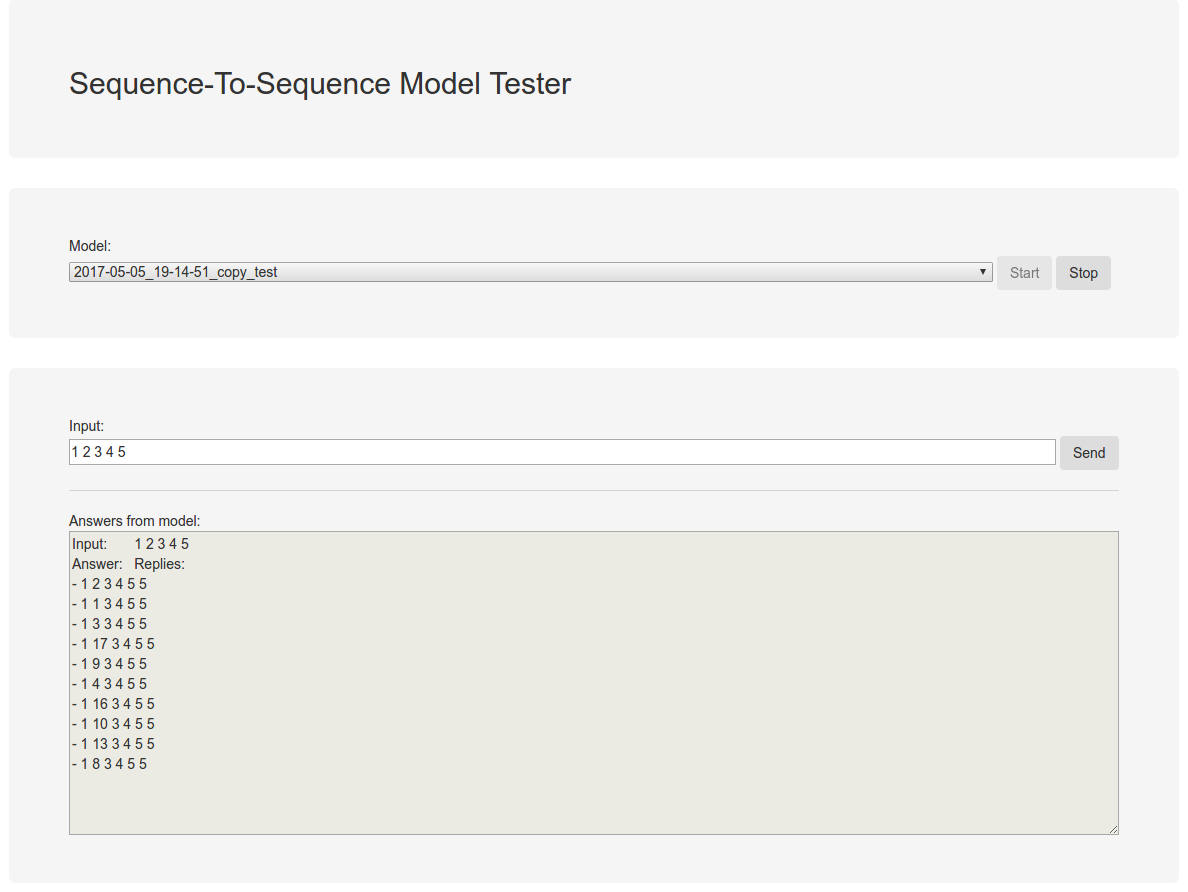
\includegraphics[width=10cm]{img/web_frontend_inference}
	\caption{Frontend showing the output when sending the sequence ``1 2 3 4 5'' to a model trained on the copy task (see chapter \ref{software_sytem:model_validation_checks}).}
\end{figure}

One last remark: Currently, there is still a bug when the user tries to end a running session and start a new one. The work around is to simply restart the entire web application.
